% --------------------------------------------------------
% DEFINIÇÕES DO DOCUMENTO
% --------------------------------------------------------

\documentclass[
	% -- opções da classe memoir --
	12pt,				% tamanho da fonte
	openright,			% capítulos começam em pág ímpar (insere página vazia caso preciso)
	oneside,			% para impressão em verso e anverso. Oposto a twoside
	a4paper,			% tamanho do papel.
	% -- opções da classe abntex2 --
	%chapter=TITLE,		% títulos de capítulos convertidos em letras maiúsculas
	%section=TITLE,		% títulos de seções convertidos em letras maiúsculas
	%subsection=TITLE,	% títulos de subseções convertidos em letras maiúsculas
	%subsubsection=TITLE,% títulos de subsubseções convertidos em letras maiúsculas
	% -- opções do pacote babel --
	english,			% idioma adicional para hifenização
	french,				% idioma adicional para hifenização
	spanish,			% idioma adicional para hifenização
	brazil,				% o último idioma é o principal do documento
	]{lib/abntex2}


% --------------------------------------------------------
% PACOTES
% --------------------------------------------------------

\usepackage{cmap}				% Mapear caracteres especiais no PDF
\usepackage{lmodern}			% Usa a fonte Latin Modern
\usepackage[T1]{fontenc}		% Selecao de codigos de fonte.
\usepackage[utf8]{inputenc}		% Codificacao do documento (conversão automática dos acentos)
\usepackage{lastpage}			% Usado pela Ficha catalográfica
\usepackage{indentfirst}		% Indenta o primeiro parágrafo de cada seção.
\usepackage{color}				% Controle das cores
\usepackage{graphicx}			% Inclusão de gráficos
\usepackage{lipsum}				% para geração de du


\let\printglossary\relax
\let\theglossary\relax
\let\endtheglossary\relax
\usepackage{lib/update-abntex}

\usepackage[brazilian,hyperpageref]{}	 % Paginas com as citações na bibl
\usepackage{microtype} 

\usepackage{silence}
%Disable all warnings issued by latex starting with "You have..."
\WarningFilter{latex}{You have requested package}
\usepackage[alf, abnt-etal-list=0 ]{lib/abntex2cite}	% Citações padrão ABNT
\usepackage[br]{lib/nicealgo}       % Pacote para criação de algoritmos
\usepackage{lib/customizacoes}      % Pacote de customizações do abntex2

\usepackage{listings}
\usepackage[normalem]{ulem} % Strikethrough package

% --------------------------------------------------------
% CONFIGURAÇÕES DE PACOTES
% --------------------------------------------------------

% Configurações do pacote listing
\renewcommand{\lstlistingname}{Código} %Mudança no caption do listing para Código
\renewcommand{\lstlistlistingname}{Lista de códigos} %Mudança no caption da lista de listings.

% Contagem de códigos sem incluir o número do capítulo
\usepackage{chngcntr}
\AtBeginDocument{\counterwithout{lstlisting}{chapter}}

% Configurações do pacote backref
\renewcommand{\familydefault}{\sfdefault}
% Usado sem a opção hyperpageref de backref
% \renewcommand{\backrefpagesname}{Citado na(s) página(s):~}
% Texto padrão antes do número das páginas
% \renewcommand{\backref}{}
% Define os textos da citação
% \renewcommand*{\backrefalt}[4]{
% 	\ifcase #1 %
% 		Nenhuma citação no texto.%
% 	\or
% 		Citado na página #2.%
% 	\else
% 		Citado #1 vezes nas páginas #2.%
% 	\fi}%


% ---
% Posiciona figuras e tabelas no topo da página quando adicionadas sozinhas
% em um página em branco. Ver https://github.com/abntex/abntex2/issues/170
\makeatletter
\setlength{\@fptop}{5pt} % Set distance from top of page to first float
\makeatother
% ---

% ---
% Possibilita criação de Quadros e Lista de quadros.
% Ver https://github.com/abntex/abntex2/issues/176
%
\newcommand{\quadroname}{Quadro}
\newcommand{\listofquadrosname}{Lista de quadros}

\newfloat[chapter]{quadro}{loq}{\quadroname}
\newlistof{listofquadros}{loq}{\listofquadrosname}
\newlistentry{quadro}{loq}{0}

% configurações para atender às regras da ABNT
\setfloatadjustment{quadro}{\centering}
\counterwithout{quadro}{chapter}
\renewcommand{\cftquadroname}{\quadroname\space} 
\renewcommand*{\cftquadroaftersnum}{\hfill--\hfill}

\setfloatlocations{quadro}{hbtp}
% ---

% --------------------------------------------------------
% INFORMAÇÕES DE DADOS PARA CAPA E FOLHA DE ROSTO
% --------------------------------------------------------

\titulo{DESENVOLVIMENTO DE UM JOGO 2D QUE ABORDA TEMAS DE SAÚDE MENTAL UTILIZANDO TÉCNICAS DE IA}
\autor{Luana Rodrigues da Silva e Lima}
\newcommand{\RA}{221015121}
\local{Bauru}
\data{Março/2025}
\orientador{Profa. Dra. Juliana da Costa Feitosa}
\coorientador{Prof. Dr. Seu Coorientador}
\instituicao{%
  Universidade Estadual Paulista ``Júlio de Mesquita Filho''
  \par
  Faculdade de Ciências
  \par
  Ciência da Computação}
\tipotrabalho{Proposta para Trabalho de Conclusão de Curso}
\preambulo{Proposta para Trabalho de Conclusão de Curso do Curso de Bacharelado em Ciência da Computação da Universidade Estadual Paulista ``Júlio de Mesquita Filho'', Faculdade de Ciências, Campus Bauru.}


% --------------------------------------------------------
% CONFIGURAÇÕES PARA O PDF FINAL
% --------------------------------------------------------

% alterando o aspecto da cor azul
\definecolor{blue}{RGB}{41,5,195}

% informações do PDF
\makeatletter
\hypersetup{
  %pagebackref=true,
  pdftitle={\@title},
  pdfauthor={\@author},
  pdfsubject={\imprimirpreambulo},
  pdfcreator={LaTeX with abnTeX2},
  pdfkeywords={abnt}{latex}{abntex}{abntex2}{trabalho acadêmico},
  colorlinks=true,    % false: boxed links; true: colored links
  linkcolor=black,    % color of internal links
  citecolor=black,    % color of links to bibliography
  filecolor=magenta,  % color of file links
  urlcolor=black,
  bookmarksdepth=4
}
\makeatother


% --------------------------------------------------------
% ESPAÇAMENTOS ENTRE LINHAS E PARÁGRAFOS
% --------------------------------------------------------

% O tamanho do parágrafo é dado por:
\setlength{\parindent}{1.3cm}

% Controle do espaçamento entre um parágrafo e outro:
\setlength{\parskip}{0.2cm}


% --------------------------------------------------------
% COMPILANDO O ÍNDICE
% --------------------------------------------------------

\makeindex

% ---
% GLOSSARIO
% ---
%\makeglossaries
% ---
% Exemplo de configurações do glossairo
\renewcommand*{\glsseeformat}[3][\seename]{\textit{#1}  
 \glsseelist{#2}}
% ---


% --------------------------------------------------------
% INÍCIO DO DOCUMENTO
% --------------------------------------------------------

\begin{document}

% Seleciona o idioma do documento (conforme pacotes do babel)
\selectlanguage{brazil}

% Retira espaço extra obsoleto entre as frases.
\frenchspacing


% --------------------------------------------------------
% ELEMENTOS PRÉ-TEXTUAIS
% --------------------------------------------------------

% Capa
% --------------------------------------------------------
% ATENÇÃO: Se você estiver tentando alterar alguns dados da capa, como o texto
% "Campus Bauru" por exemplo, dê uma procurada no arquivo lib/customizacoes.sty
% próximo à linha 59.
% --------------------------------------------------------
\imprimircapaproposta

% Folha de rosto
% (o * indica que haverá a ficha bibliográfica)
\imprimirfolhaderosto



% --------------------------------------------------------
% SUMÁRIO
% --------------------------------------------------------

% inserir o sumario
\pdfbookmark[0]{\contentsname}{toc}
\tableofcontents*
\cleardoublepage


% --------------------------------------------------------
% ELEMENTOS TEXTUAIS
% --------------------------------------------------------

\pagestyle{simple}

% Arquivos .tex do texto, podendo ser escritos em um único arquivo ou divididos da forma desejada
\chapter{Introdução}
\label{c.introducao}


A saúde mental é um componente crítico do bem-estar geral e ela se manifesta de forma variável em cada pessoa, de maneira muito parecida com a saúde física \cite{deleene}. Ao longo da vida, diversos determinantes contribuem para proteger, prejudicar ou deixar mais vulnerável a saúde mental do ser humano, como fatores psicológicos e biológicos individuais, circunstâncias sociais  e ambientes desfavoráveis \cite{world_2022}. 

Esse tema ganhou importância e visibilidade recentemente com a divulgação da Agenda de Desenvolvimento Sustentável 2030 da Organização das Nações Unidas (ONU), pois pela primeira vez as metas incluíram saúde mental de maneira explícita. No Objetivo de Desenvolvimento Sustentável (ODS) 3.4 foi estabelecida a meta de "promover a saúde mental e o bem-estar". Esse tema possui grandes impactos na qualidade de vida humana, pois pesquisas mostraram que condições de saúde mental são responsáveis por 13\% dos anos vividos com incapacidade e perdidos por morte prematura \cite{heymann_sprague_2023}; em 2019, uma a cada oito pessoas viveram com algum transtorno mental, um número que aumentou consideravelmente por causa da pandemia do COVID-19 \cite{mentalDisorders_2022}. 

Jogos Sérios são jogos cujo propósito não é apenas entretenimento, mas também a exploração ativa de problemas sociais \cite{abt1987serious}. Eles são utilizados para diversas finalidades: auxiliar no processo educacional, ajudar pacientes a entender sua condição atual e sua reabilitação, promover a conscientização do público para problemas psicológicos e emocionais, etc. Além disso, uma categoria recente de jogos vem ganhando destaque: jogos empáticos. Esses jogos priorizam, através de mecânicas, trazer a experiência de como é estar no lugar de outra pessoa. O aspecto interativo que os jogos trazem permite que o jogador participe ativamente do conteúdo mostrado, não sendo apenas observadores passivos, mas sim participantes afetados pelos eventos do universo. Dessa forma, é possível fazer com que o usuário tenha interesse em tópicos relacionados à saúde mental (como o luto e transtornos mentais) e ter uma visão mais empática sobre esse tema \cite{10.1145/3638067.3638104}.

O desenvolvimento de jogos 2D envolve a criação de um jogo que exista num espaço bidimensional, onde todos os componentes são representados usando dois eixos. De acordo com \citeonline{article}, apesar de estarmos numa era dominada por gráficos 3D, os jogos 2D mantêm sua popularidade. Isso ocorre pois são mais baratos de serem produzidos, sendo o melhor mercado para um desenvolvedor independente \cite{book}.

A Inteligência Artificial (IA) é um campo rico e diverso, que possui aplicabilidade em várias vertentes como automóveis, saúde, entretenimento, educação, segurança, entre outras. A IA foca em aprender com experiências e alterar seu processamento e comportamento baseado em seu aprendizado. Além disso, é considerada a próxima revolução industrial na área de entretenimento e também é capaz de aumentar a eficiência automatizando numerosas tarefas repetitivas \cite{articleIAEntretenimento}. Na indústria de jogos, a IA é utilizada para  gerar comportamentos responsivos, adaptativos e inteligentes para personagens não jogáveis (em inglês, NPCs) \cite{IA_jogos}. De acordo com \citeonline{jorapur2024evolution}, ela também é implementada para adaptar a história dependendo do comportamento do jogador, para criação de diferentes conteúdos do jogo como níveis e mundos infinitos e para ajustar a dificuldade de acordo com a performance do player. Além disso, é usada para fazer animações de personagem \cite{xian2023automated}.

Nesse contexto, o projeto visa desenvolver um jogo sério 2D que utiliza IA para fazer as animações dos personagens, e que aborda temas de saúde mental para trazer uma visão mais empática e conscientizar sobre esse assunto. 







 
 
  
\chapter{Problema}
\label{c.problema}

De acordo com a Organização Mundial da Saúde (OMS), a saúde mental é extremamente importante para todos. Globalmente, as necessidades de saúde mental são altas, mas as respostas são insuficientes e inadequadas \cite{world}.

Transtornos mentais, em muitos casos, não são facilmente reconhecíveis baseados na aparência e comportamento externo de uma pessoa. Assim, aqueles afetados por isso sofrem com a falta de empatia e de aceitação, sendo alvos de discriminação e psicofobia (preconceito direcionado a pessoas com transtornos mentais) \cite{kasdorf_2023}. O estigma é encontrado no ambiente de trabalho, familiar e escolar, fazendo com que o indivíduo se retraia, seja desencorajado a discutir sobre sua saúde mental, desenvolva mecanismos de enfrentamento prejudiciais e tenha um agravamento dos sintomas. Além disso, existe também a  auto estigmatização, que é a internalização de crenças negativas sobre si mesmo e auto discriminação \cite{Roma_2024}.

A IA tem feito contribuições significativas para os jogos digitais, porém sua aplicação em animações 2D é pouco explorada. As ferramentas de IA para animação atualmente têm como alvo especificamente vídeos tridimensionais, que não têm um controle efetivo sobre a aleatoriedade \cite{articleIAanima}. 








\chapter{Justificativa}
\label{c.justificativa}

 A mídia em geral é uma fonte extremamente importante de conhecimento sobre transtornos, com os jogos sendo um dos tipos mais impactantes de mídia digital. Essa representação de assuntos relacionados à saúde mental afeta as atitudes e crenças do público. No mundo dos jogos digitais, por exemplo, é muito comum a representação de transtornos mentais, porém ela é acompanhada de discriminação e estigmatização \cite{kasdorf_2023}. 

 Conforme citado, o uso da IA nas animações 2D foi muito pouco explorado, fazendo com que possivelmente essa tecnologia tenha o potencial de revolucionar o processo complexo de produção de animação 2D \cite{articleIAanima}. Automatizando o processo, o tempo e o esforço são reduzidos, sendo possível produzir animações de alta qualidade mais rapidamente e com um custo menor \cite{xian2023automated}.

Diante do contexto apresentado, é necessário encontrar maneiras de combater os estigmas e preconceitos envolvidos ao redor do tema de saúde mental, além de ser necessário disseminar mais sobre o assunto e sua importância. Para isso, a proposta desse projeto é desenvolver um jogo sério 2D que aborda temas de saúde mental de forma mais subjetiva, cujo jogador controlará um personagem que passa por problemas psicológicos e emocionais. Além disso, será usada uma IA para fazer as animações do jogo e analisar o potencial dessa tecnologia para o auxílio na produção de animações 2D. O projeto também proporciona uma oportunidade para praticar os conhecimentos de Computação Gráfica e Engenharia de Software, contribuindo para a formação acadêmica.


\chapter{Objetivos}
\label{c.objetivos}

\section{Objetivos Gerais}
\label{s.gerais}

Desenvolver e implementar um jogo 2D utilizando técnicas de IA para conscientização sobre temas de saúde mental. 


\section{Objetivos Específicos}
\label{s.especificos}

\begin{itemize}
\item Utilizar técnicas de Engenharia de Software para desenvolvimento do jogo de forma organizada;
\item Desenvolver um Game Design Document (GDD) estruturando o jogo;
\item Modelar as cenas, cenários e personagens do jogo;
\item Programar mecânicas que representem de forma responsável o estado da saúde mental do personagem;
\item Pesquisar métodos para lidar com situações de estresse e trauma para sua implementação no jogo.
\item Estudar técnicas de IA aplicáveis ao problema
\item Desenvolver e treinar a IA para auxílio na produção de animações 2D; e
\item Verificar a eficácia e potencial da IA em animar cenas 2D;
\end{itemize}
\chapter{Metodologia}
\label{c.metodologia}

%   ---------------------   EDITAR PARA O QUE REALMENTE ACONTECEU -------------------

Inicialmente, será elaborado o documento GDD e o projeto de arquitetura de software, que contribuem para a organização da estrutura, roteiro, cenários e personagens do jogo. Isso será feito de forma paralela com um levantamento bibliográfico mais aprofundado sobre saúde mental, traumas, problemas emocionais, distúrbios mentais e mecanismos de enfrentamento saudáveis.

Depois que os documentos forem elaborados, será iniciado o desenvolvimento do jogo, desenhando o ambiente de cada cena e programando cada mecânica. Quando o levantamento bibliográfico sobre saúde mental for concluído, uma pesquisa sobre modelos de IA para animação será feita, analisando quais as técnicas utilizadas por cada um, as vantagens, as desvantagens e o foco. Após a pesquisa, será escolhido um modelo para ser treinado, implementado e modificado conforme necessário. O treinamento será feito de forma paralela com o desenvolvimento do jogo. Após a IA ter sido treinada, ela será utilizada para fazer as animações dos personagens do jogo. Durante o estudo, treinamento e implementação do modelo da IA, será feita uma análise de como o modelo ajuda no cenário de animações 2D, documentando qualquer modificação feita. Ao longo do desenvolvimento, serão realizados diversos testes para verificar se o comportamento está de acordo com o esperado. 

A partir do momento em que o jogo for concluído, serão realizados testes finais para verificar o funcionamento correto de todos os elementos, fazendo ajustes se necessário. O planejamento da ordem em que cada atividade será realizada é demonstrado pela Figura \ref{f.Diagrama}.

\begin{figure}[htbp]
	\caption{\small Fluxograma das etapas}
	\centering
	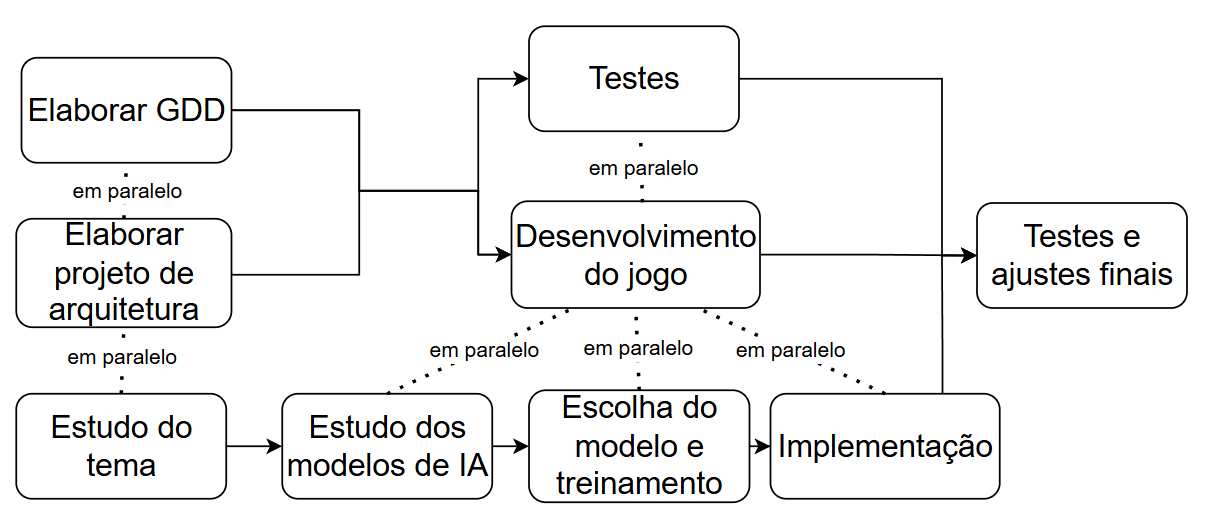
\includegraphics[width=1\linewidth]{figs/Diagrama.PNG}
	\label{f.Diagrama}
	\legend{\small Fonte: Elaborada pela autora.}
\end{figure}

%   ------------------------------------------------------------------------
\FloatBarrier
\section{Metodologia de desenvolvimento do jogo}
\label{s.jogo}

\FloatBarrier
\section{Metodologia de Análise das Ferramentas de IA}
\label{s.ia}


Para conduzir a análise comparativa das ferramentas de IA, a metodologia foi estruturada em etapas, partindo de uma seleção ampla de ferramentas até uma avaliação aprofundada das mais promissoras.

Inicialmente, foram estabelecidos os seguintes critérios de seleção para a escolha de ferramentas:

\begin{itemize}
\item Capacidade de criar vídeos ou imagens que pudessem ser usados para a animação 2D;
\item Disponibilidade de um modelo de acesso gratuito, ainda que com limitações de uso;
\item Possibilidade de usar uma imagem pré-existente (do personagem ou objeto) como referência, para consistência visual; e
\item Acessível para um usuário sem conhecimento aprofundado na ferramenta.
\end{itemize}

%------------------------ CHECAR SE NÃO OLHOU NENHUMA NOVA NÃO MENCIONADA ----------------
Com base nesses critérios, foram selecionados os seguintes softwares como candidatos para a produção de animação 2D: CGDream \cite{cgdream_2025}, ChatGPT \cite{chatgpt_2025}, OpenArtAI\cite{openArtai_2025}, geminiPro \cite{gemini_2025}, God Mode AI \cite{godmodeanimation2024}, PixelLab \cite{pixelLab}, PixieHaus \cite{pixie.haus_2025}, Rosebud AI \cite{rosebud}, Animated Drawings \cite{animatedDrawings}, Vidu \cite{viduai_2024}, AI Sprite Sheet Maker \cite{segmind} e SpriteSheetGPT \cite{spritesheetgpt-free}. 


O processo de análise foi dividido em duas fases. A primeira fase consistiu em uma análise geral de cada ferramenta, verificando os recursos grátis disponíveis, as opções de customização existentes e a capacidade de gerar uma animação 2D útil para o jogo em desenvolvimento a partir de um sprite de referência. Essa triagem inicial permitiu descartar algumas ferramentas que provaram não ser capazes de alcançar o resultado desejado, sobrando apenas as candidatas mais promissoras. Um desafio descoberto nesta etapa foi a limitação de uso do modelo gratuito de muitas plataformas, o que restringiu o número de testes comparativos e reduziu o número de gerações.

Na segunda fase, foi realizado um aprofundamento das ferramentas restantes. Foram conduzidos testes iterativos com diversos prompts (a maioria em inglês para melhores resultados) e imagens de referências nas plataformas que não possuíam um limite para o uso gratuito, ou este era muito alto. Para as plataformas mais restritas, os resultados que chegavam mais perto do desejado eram usados como referência para os outros softwares. As animações satisfatórias foram implementadas no jogo, com o uso de ferramentas auxiliares para converter ou ajustar o formato do arquivo e para pequenas edições na imagem.

%------------- CHECAR SE NÃO CRIOU NENHUMA ANIMAÇÃO NOVA NÃO MENCIONADA ----------------
Foram criadas animações com IA para alguns elementos do jogo: o personagem Pablo (Figura \ref{fig:Pablo}), que realiza as ações de andar, pular, virar de costas e sentar; a personagem Luz; e a porta (Figuras \ref{fig:portaA}, \ref{fig:portaB}) e \ref{fig:portaC}, que executa os movimentos de abrir e fechar. Os resultados adequados foram implementados no jogo.


\begin{figure}[htbp]
    \centering
    \caption{\small Sprite do Pablo}
    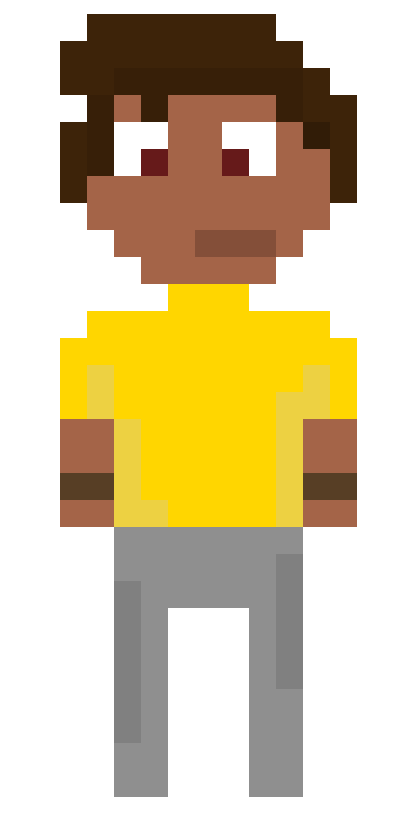
\includegraphics[width=0.3\linewidth]{figs/sprites/Pablo.PNG}
    \label{fig:Pablo}
    \legend{\small Fonte: Elaborada pela autora.}
\end{figure}


\begin{figure}[htbp]
    \centering
    \caption{\small Sprite da Luz}
    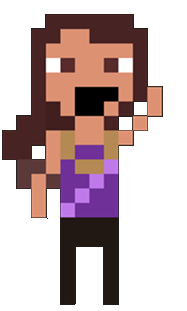
\includegraphics[width=0.3\linewidth]{figs/sprites/irma.PNG}
    \label{fig:Luz}
    \legend{\small Fonte: Elaborada pela autora.}
\end{figure}


\begin{figure}[htbp]
    \centering
    \begin{minipage}{0.45\textwidth}
    \caption{\small Sprite da porta A em front view (vista frontal, em inglês)}
    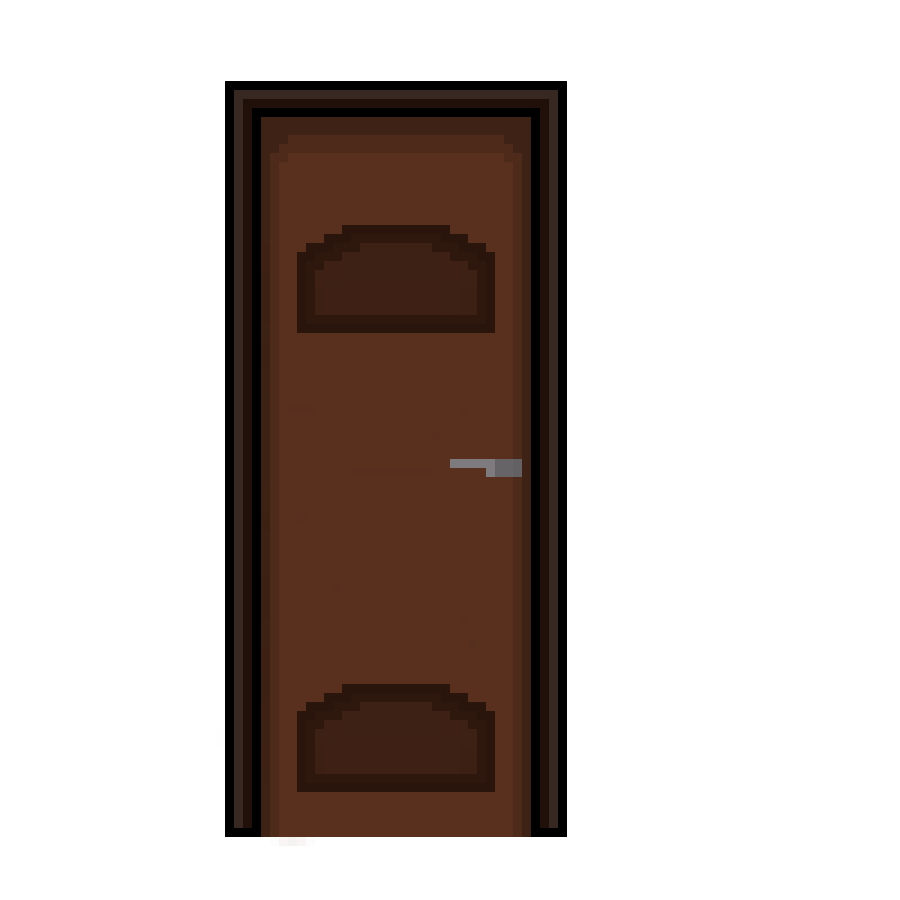
\includegraphics[width=1\linewidth]{figs/sprites/Porta front view.png}
    \label{fig:portaA}
    \legend{\small Fonte: Elaborada pela autora.}
    \end{minipage}\hfill
    \begin{minipage}{0.45\textwidth}
    \caption{\small Sprite da porta B em side view (vista lateral, em inglês)}
    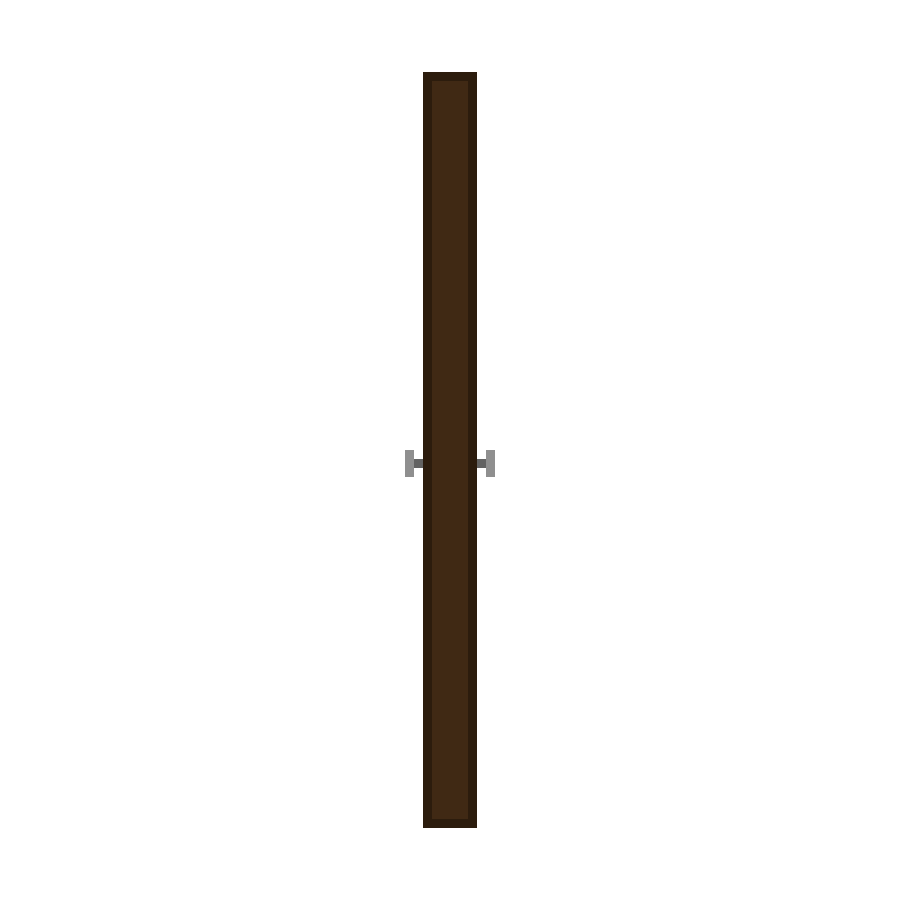
\includegraphics[width=1\linewidth]{figs/sprites/Porta side view.png}
    \label{fig:portaB}
    \legend{\small Fonte: Elaborada pela autora.}
    \end{minipage}\hfill
\end{figure}


\begin{figure}[htbp]
    \centering
    \caption{\small Sprites da porta C}
    \label{fig:portaC}
    \begin{subfigure}{0.45\textwidth}
    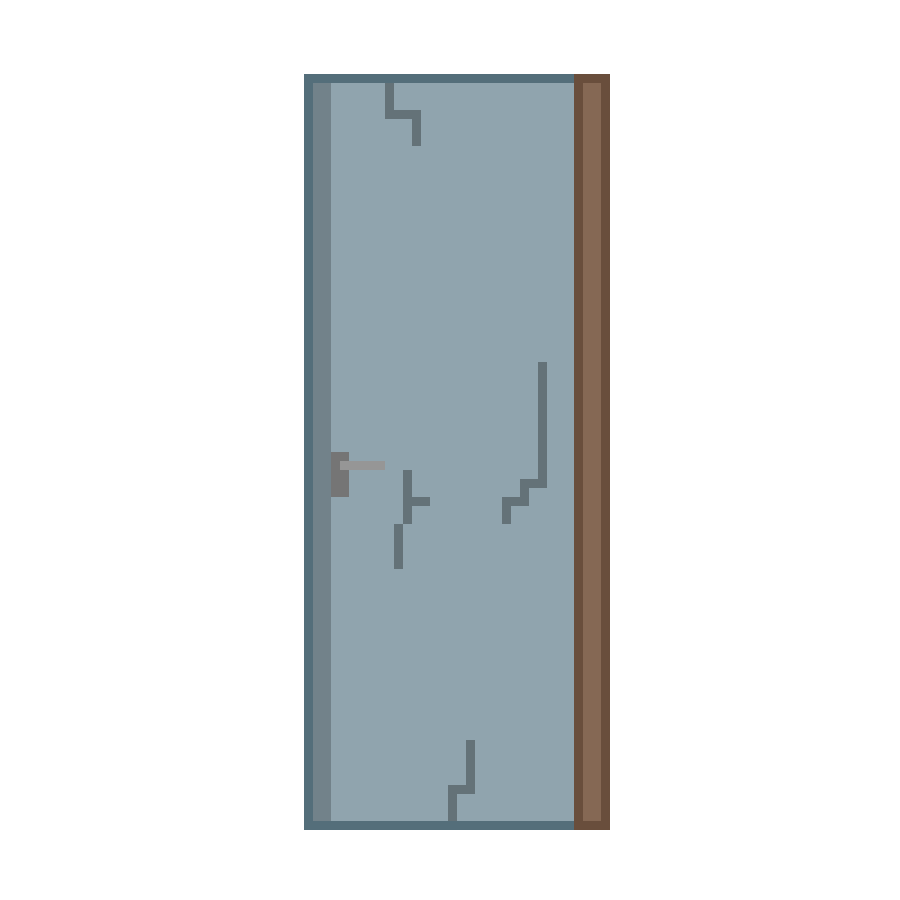
\includegraphics[width=1\linewidth]{figs/sprites/referencia_porta_tutorial (1).png}
    \caption{\small Sprite da porta C aberta em side view}
    \label{fig:portaCAberto}
    \end{subfigure}\hfill
    \begin{subfigure}{0.45\textwidth}
    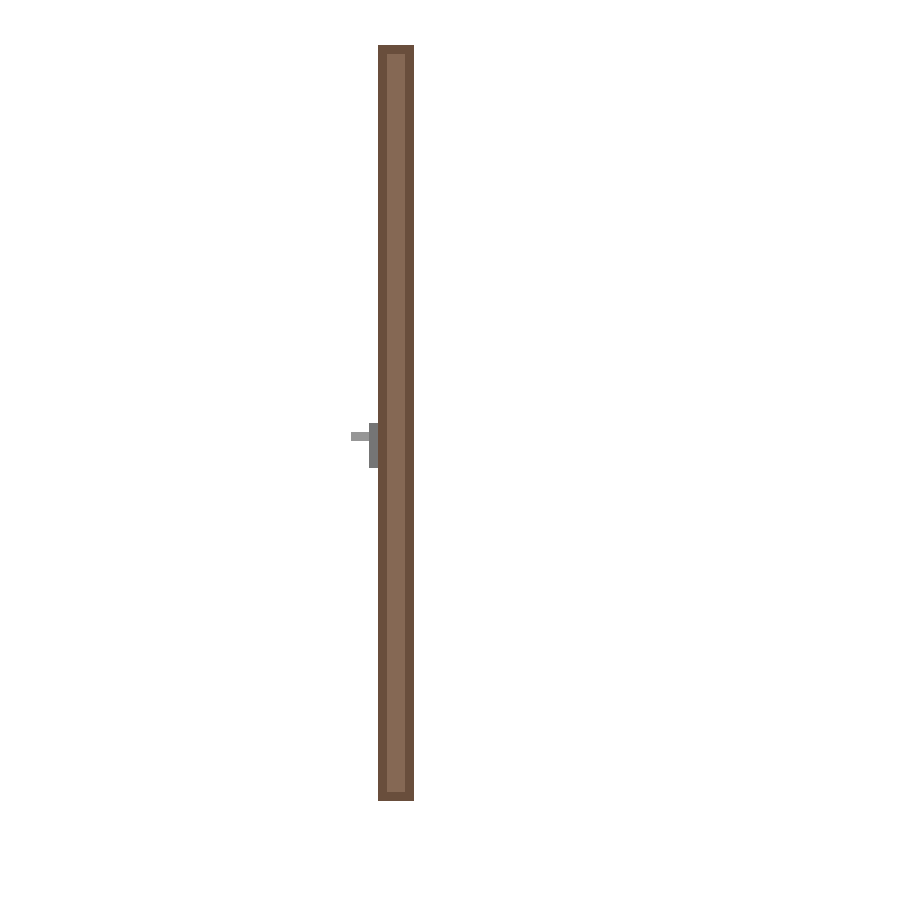
\includegraphics[width=1\linewidth]{figs/sprites/referencia_porta_tutorial (2).png}
    \caption{\small Sprite da porta C fechada em side view}
    \label{fig:portaCFechado}

    \end{subfigure}\hfill
    \legend{\small Fonte: Elaborada pela autora.}
\end{figure}

Ao final do processo, as ferramentas mais satisfatórias serão comparadas e avaliadas pelos seguintes critérios:

\begin{itemize}
\item Foco em 2D;
\item Consistência com o estilo e cores da imagem de referência;
\item Facilidade de uso e curva de aprendizagem;
\item Precisão de movimento e fidelidade ao prompt;
\item Qualidade estética;
\item Nível de customização;
\item Eficiência;
\item Capacidade de produzir resultado pixel perfect (todos os pixels tem o mesmo tamanho); e
\item Capacidade de edição e refinamento do material gerado.
\end{itemize}

\chapter{Cronograma}
\label{c.cronograma}

O projeto foi dividido nas seguintes etapas:

\begin{itemize}
    \item Estudo do tema;
    \item Elaboração do GDD;
    \item Elaboração do projeto de arquitetura;
    \item Estudo de modelos de IA;
    \item Escolha do modelo de IA e treinamento;
    \item Implementação do modelo de IA;
    \item Testes e adaptações necessárias;
    \item Desenvolvimento do jogo;
    \item Testes e revisões finais; e
    \item Redação da monografia.
\end{itemize}  

O momento de realização de cada uma dessas etapas é apresentado no Quadro \ref{cronograma}.\\


\begin{quadro}
    \centering
    \caption{Cronograma}
    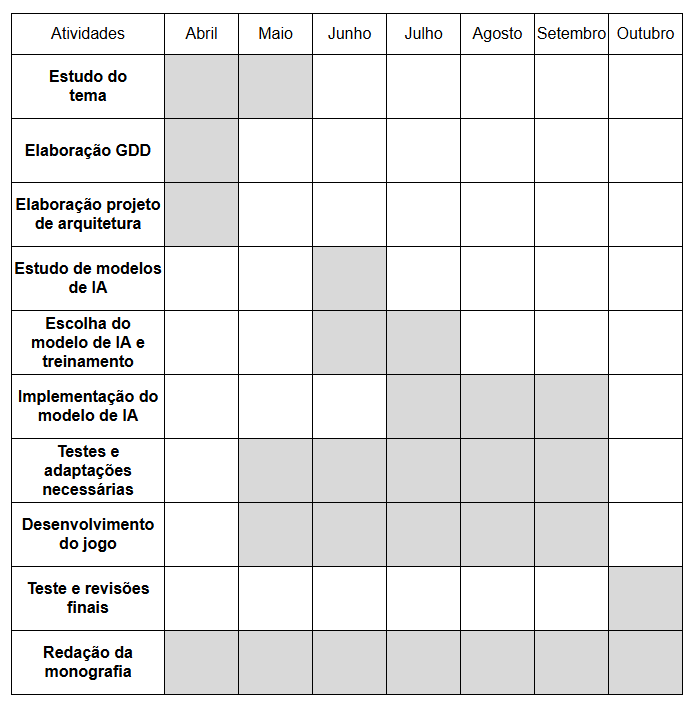
\includegraphics[width=1\linewidth]{figs/cronograma.PNG}
    \label{cronograma}
    \fonte{Elaborado pela autora.}
\end{quadro}




% --------------------------------------------------------
% REFERÊNCIAS BIBLIOGRÁFICAS
% --------------------------------------------------------

\bibliography{chapters/referencias}


% --------------------------------------------------------
% ÍNDICE REMISSIVO
% --------------------------------------------------------

%\printindex


% --------------------------------------------------------
% FINAL DO DOCUMENTO
% --------------------------------------------------------

\end{document}